\chapter{Ausblick}

\section{Erweiterungsvorschl�ge}
In Abschnitt ref{Kunden, Dienstleister und Schichtenmodelle} wurde zwar gesagt,
dass es aus Kostengr�nden nicht m�glich ist, eine Middleware zur Verwaltung der
Datenbankzugriffe zu erwerben, jedoch w�re zu �berlegen, ob es nicht sinnvoll
ist eine eigene Mittelschicht zu entwerfen. Sie muss nicht in allen
Einzelheiten vollst�ndig sein und mehrere Datenbank-Treiber unterst�tzen.
Vielmehr gen�gt, es wenn sie den Anforderungen entsprechend erweiterbar ist und
vorerst die Grundoperationen realisiert. Da eine Kommunikation mit CORBA und
RMI im Projekt vorgesehen ist, w�re nach deren Umsetzung das Einf�gen dieser
Mittelschicht ein gute L�sung, um die momentan aufgebl�hten Fat-Clients in
Thin-Clients zu konvertieren, welche dann haupts�chlich nur noch Domain- und
Pr�sentionslogik enthalten. Das erspart dem Anwender auch die Konfiguration der
Datenbankserveranbindung und vereinfacht einen m�glichen Lokationswechsel der
Datenbank.


\section{Einsatzgebiete von Resemedicinae}

\subsection{Zwei Anwendungsbeispiele}
Die wesentliche Neuerung bei Resmedicinae ist, die Vorteile des Internets und
verteilter Anwendungen auch f�r Patientenkarteien nutzbar zu machen.
Patientendaten ein und der selben Person k�nnen an verschiedenen Stellen der
Welt gleichzeitig abgerufen und bearbeitet werden. So entfallen langwierige
Wartezeiten beim �berweisen eines Patienten an einen Facharzt, da das versenden
der Patientenakte entf�llt. Alle notwendigen Informationen werden in einer
Zentralen Datenbank abgespeichert. Die Transaktionen erfolgen unter Beachtung
von � X Absatz U des Bundesdatenschutzgesetz (BDSG), wonach keine medizinischen
Daten im Internet gespeichert werden d�rfen.

\begin{figure}[ht]
    \begin{center}
       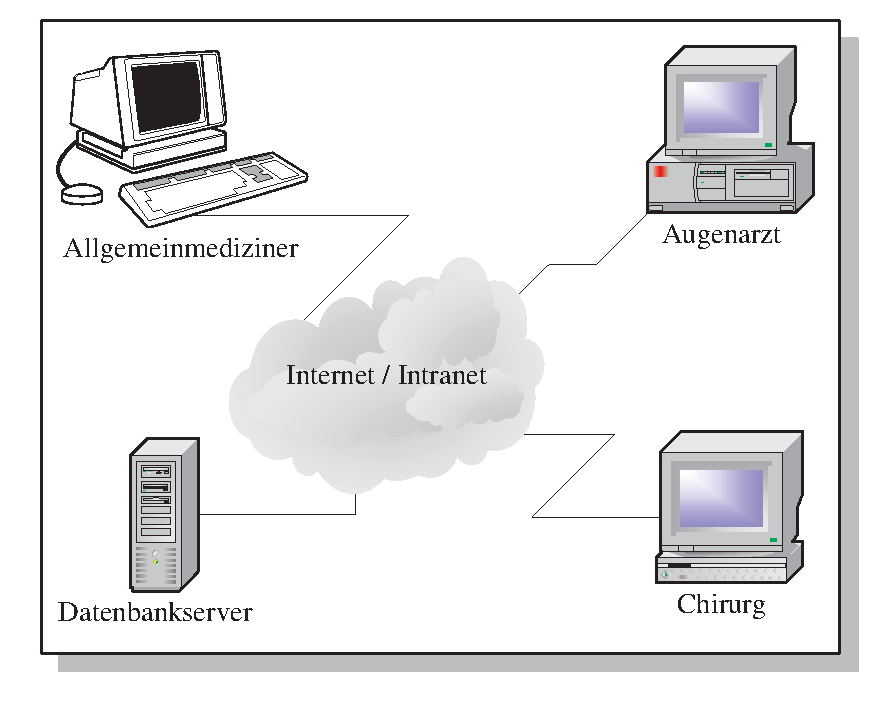
\includegraphics[scale=0.8]{Bilder/Anwendungen1_Internet.eps}
       \caption{Einsatz von Resmedicinae im Internet}
       \label{fig:Einsatz von Resmedicinae im Internet}
    \end{center}
\end{figure}

\newpage

Eine andere M�glichkeit w�re, Resmedicinae einrichtungsintern beschr�nkt zu
nutzen, beispielsweise innerhalb eines Krankenhauses, um lediglich interne
Daten zu verwalten. Diese Daten k�nnen aber ebenso, wie in erstem Beispiel, von
jedem Arzt an einem Terminal abgerufen und modifiziert werden. Denkbar w�re
auch, die �rzte mit einer Art Handhelt (einer tragbaren Rechnerversion)
auszustatten, der �ber Funk mit der Datenbank des Krankenhauses verbunden ist.
Dabei darf das Sende- / Empfangssignal energetisch nur ein sehr niedriges
Niveau erreichen, um die empfindlichen medizinischen Apparaturen nicht zu
beeinflussen, wie es beispielsweise bei Handys der Fall sein kann. Es sind
jedoch nur sehr kurze Distanzen innerhalb innerhalb der Einrichtung zu
�berwinden und deshalb keine starken Signale von n�ten.\\
Somit besteht im Bereich des Funknetzes eine Ortsunabh�ngigkeit. Dem Arzt
bleibt es erspart nach einzelnen Patientenbesuchen einen Terminal oder eine
Workstation aufsuchen zu m�ssen, sondern kann seine elektronischen Akten gleich
an Ort und Stelle verwalten.

\begin{figure}[ht]
    \begin{center}
       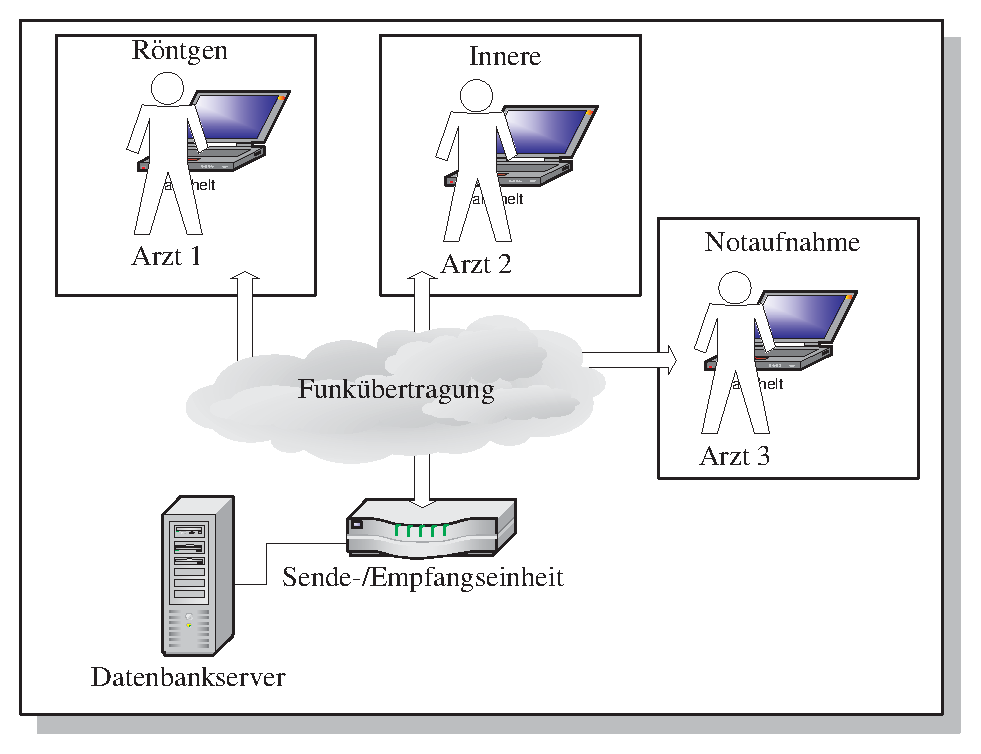
\includegraphics[scale=0.8]{Bilder/Anwendungen2_Krankenhaus.eps}
       \caption{Einsatz von Resmedicinae einrichtungsintern}
       \label{fig:Einrichtungsinterner Einsatz von Resmedicinae}
    \end{center}
\end{figure}
